%!TEX root = ../../super_main.tex

\section{Sensor Providers}
\label{sec:sensor_providers}

We have implemented a threaded abstraction over the different data sources that the system should utilize in order to gather context for the labels that will eventually be combined to form the output training data for the system. The abstraction is threaded because we want the Android application to be able to gather information from multiple sources concurrently. This is done in order to make sure that the gathered data is obtained temporally close to when the label for the data was obtained. 

\subsection{Temporality}

\subsubsection{}

\subsubsection{}

\subsubsection{}

\begin{figure}[!htbp]
    \centering
    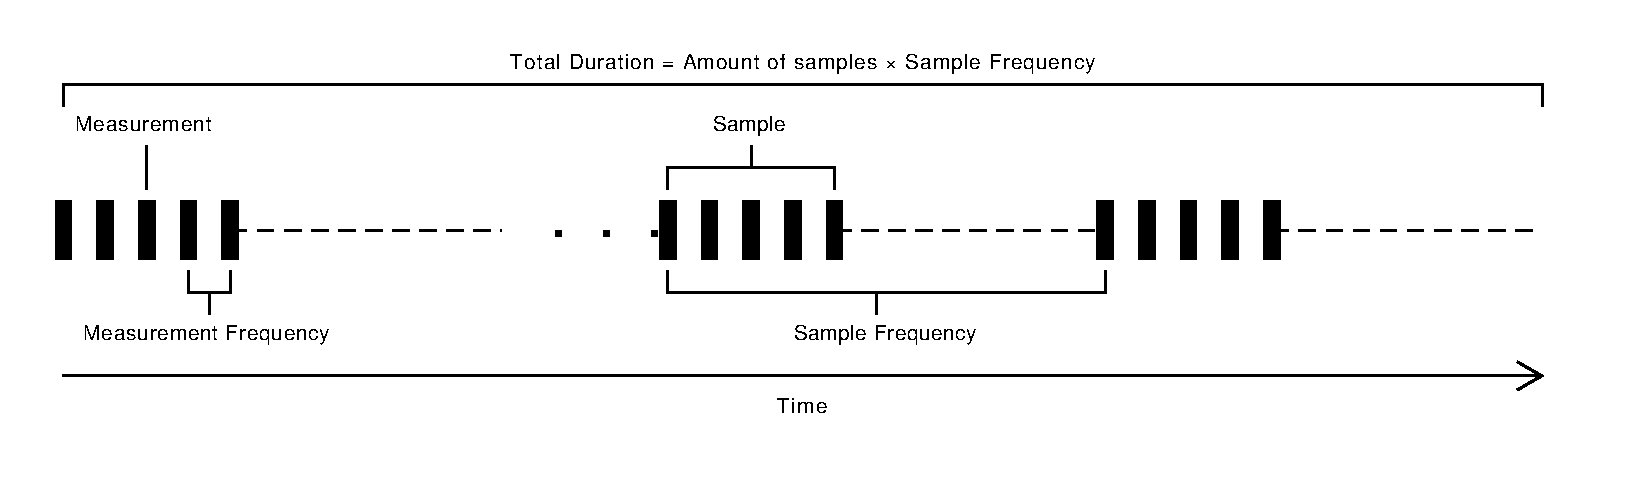
\includegraphics[width=\textwidth]{unsorted/sample_temporality}
    \caption{Overview of sample and measurement temporality.}
    \label{fig:sample_temporality}
\end{figure}

\subsection{Implementation}

% Future<T> Objects
% 

% \lstinputlisting[
%    style = java,
%    caption = {Property similarity on a component.},
%    label = {lst:attribute_difference},
%]{content/implementation/annotation/attribute_difference.java}